\chapter{\textbf{Resultados}} % Este comando é utilizado para criar capítulos
\sloppy % Corrige estouro de linhas

\section{Aplicativo}

Todo o processo de construção do aplicativo foi baseado na metodologia utilizada na disciplina de Laboratório de Engenharia de \textit{Software} \cite{rupLes}. Para tanto, foram realizadas as seguintes etapas:

\subsection{Levantar Requisitos (Visão Geral)}

Nesta etapa foi realizado um levantamento de funcionalidades básicas necessárias junto a empresa responsável pelo gerenciamento dos dados dos alunos. A partir desta, foi elaborado uma descrição geral sobre o escopo do aplicativo.

\subsection{Elaborar Modelo Conceitual}

A construção do modelo conceitual foi baseada no levantamento realizado na etapa anterior, levando em consideração as informações disponibilizadas pela base de dados cedida, conforme a figura \ref{figura:modelo_conceitual}.

\begin{figure}[H]
	\caption{Modelo Conceitual.}
	\centering % para centralizarmos a figura
	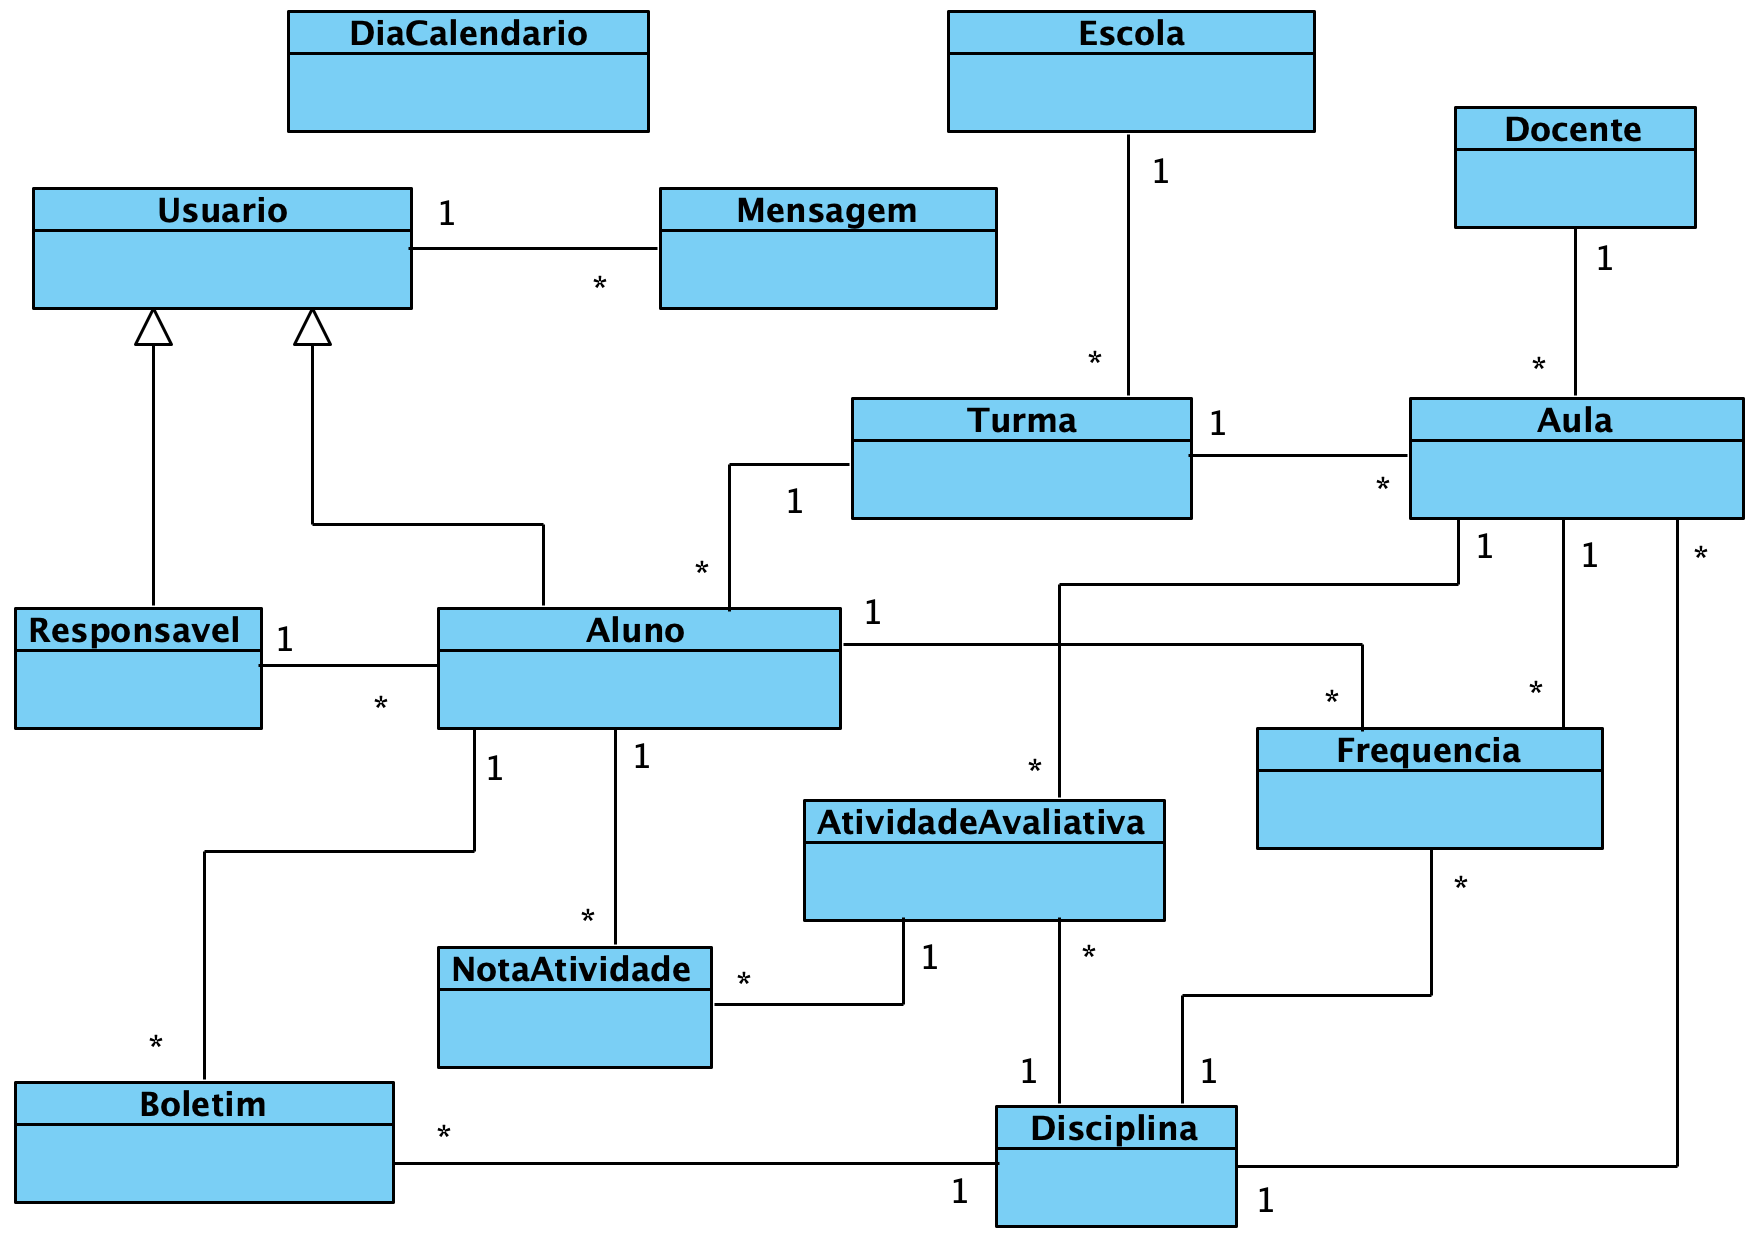
\includegraphics[width=13.5cm]{resources/modelo_conceitual.png} % leia abaixo
	\label{figura:modelo_conceitual}
	\captionsetup{singlelinecheck = false, format= hang, justification=raggedright, labelsep=space, width=13.7cm}
	\caption*{\footnotesize Fonte: O Autor.}
\end{figure}

\subsection{Levantar Requisitos}

Nesta etapa foi produzido o documento de requisitos. Ao todo, foram identificados 15 requisitos, sendo 12 de processos de negócio e 3 de listagens. Todos os requisitos foram definidos a partir de reuniões realizadas com a empresa responsável por ceder os dados.

\subsection{Organizar Requisitos}

Nesta etapa, os requisitos foram organizados entre as categorias: processos de negócios e listagens/relatórios.

Os requisitos de processos de negócio foram, respectivamente: entrar no sistema; sair do sistema; enviar cliques do responsável; listar horários de aula por id do aluno; listar atividades avaliativas por id do aluno, período e trimestre; listar disciplinas de atividades avaliativas por id do aluno e período; listar boletim por id do aluno e período; listar frequências por id do aluno, id da disciplina e período; selecionar aluno por id; listar alunos por responsável e ano letivo; listar calendário acadêmico; listar mensagens por usuário.

Os requisitos de listagem foram, respectivamente: listar total de frequências por id do aluno, período e id da disciplina; listar disciplinas de frequências por id do aluno e período; listar total de faltas por id do aluno e período.

\subsection{Elaborar diagrama de classes de projeto}

Nesta etapa foi elaborado o diagrama de classes de projeto, considerando os dados a serem utilizados no aplicativo, levantados no documento de requisitos.

\begin{figure}[H]
	\caption{Diagrama de Classe.}
	\centering % para centralizarmos a figura
	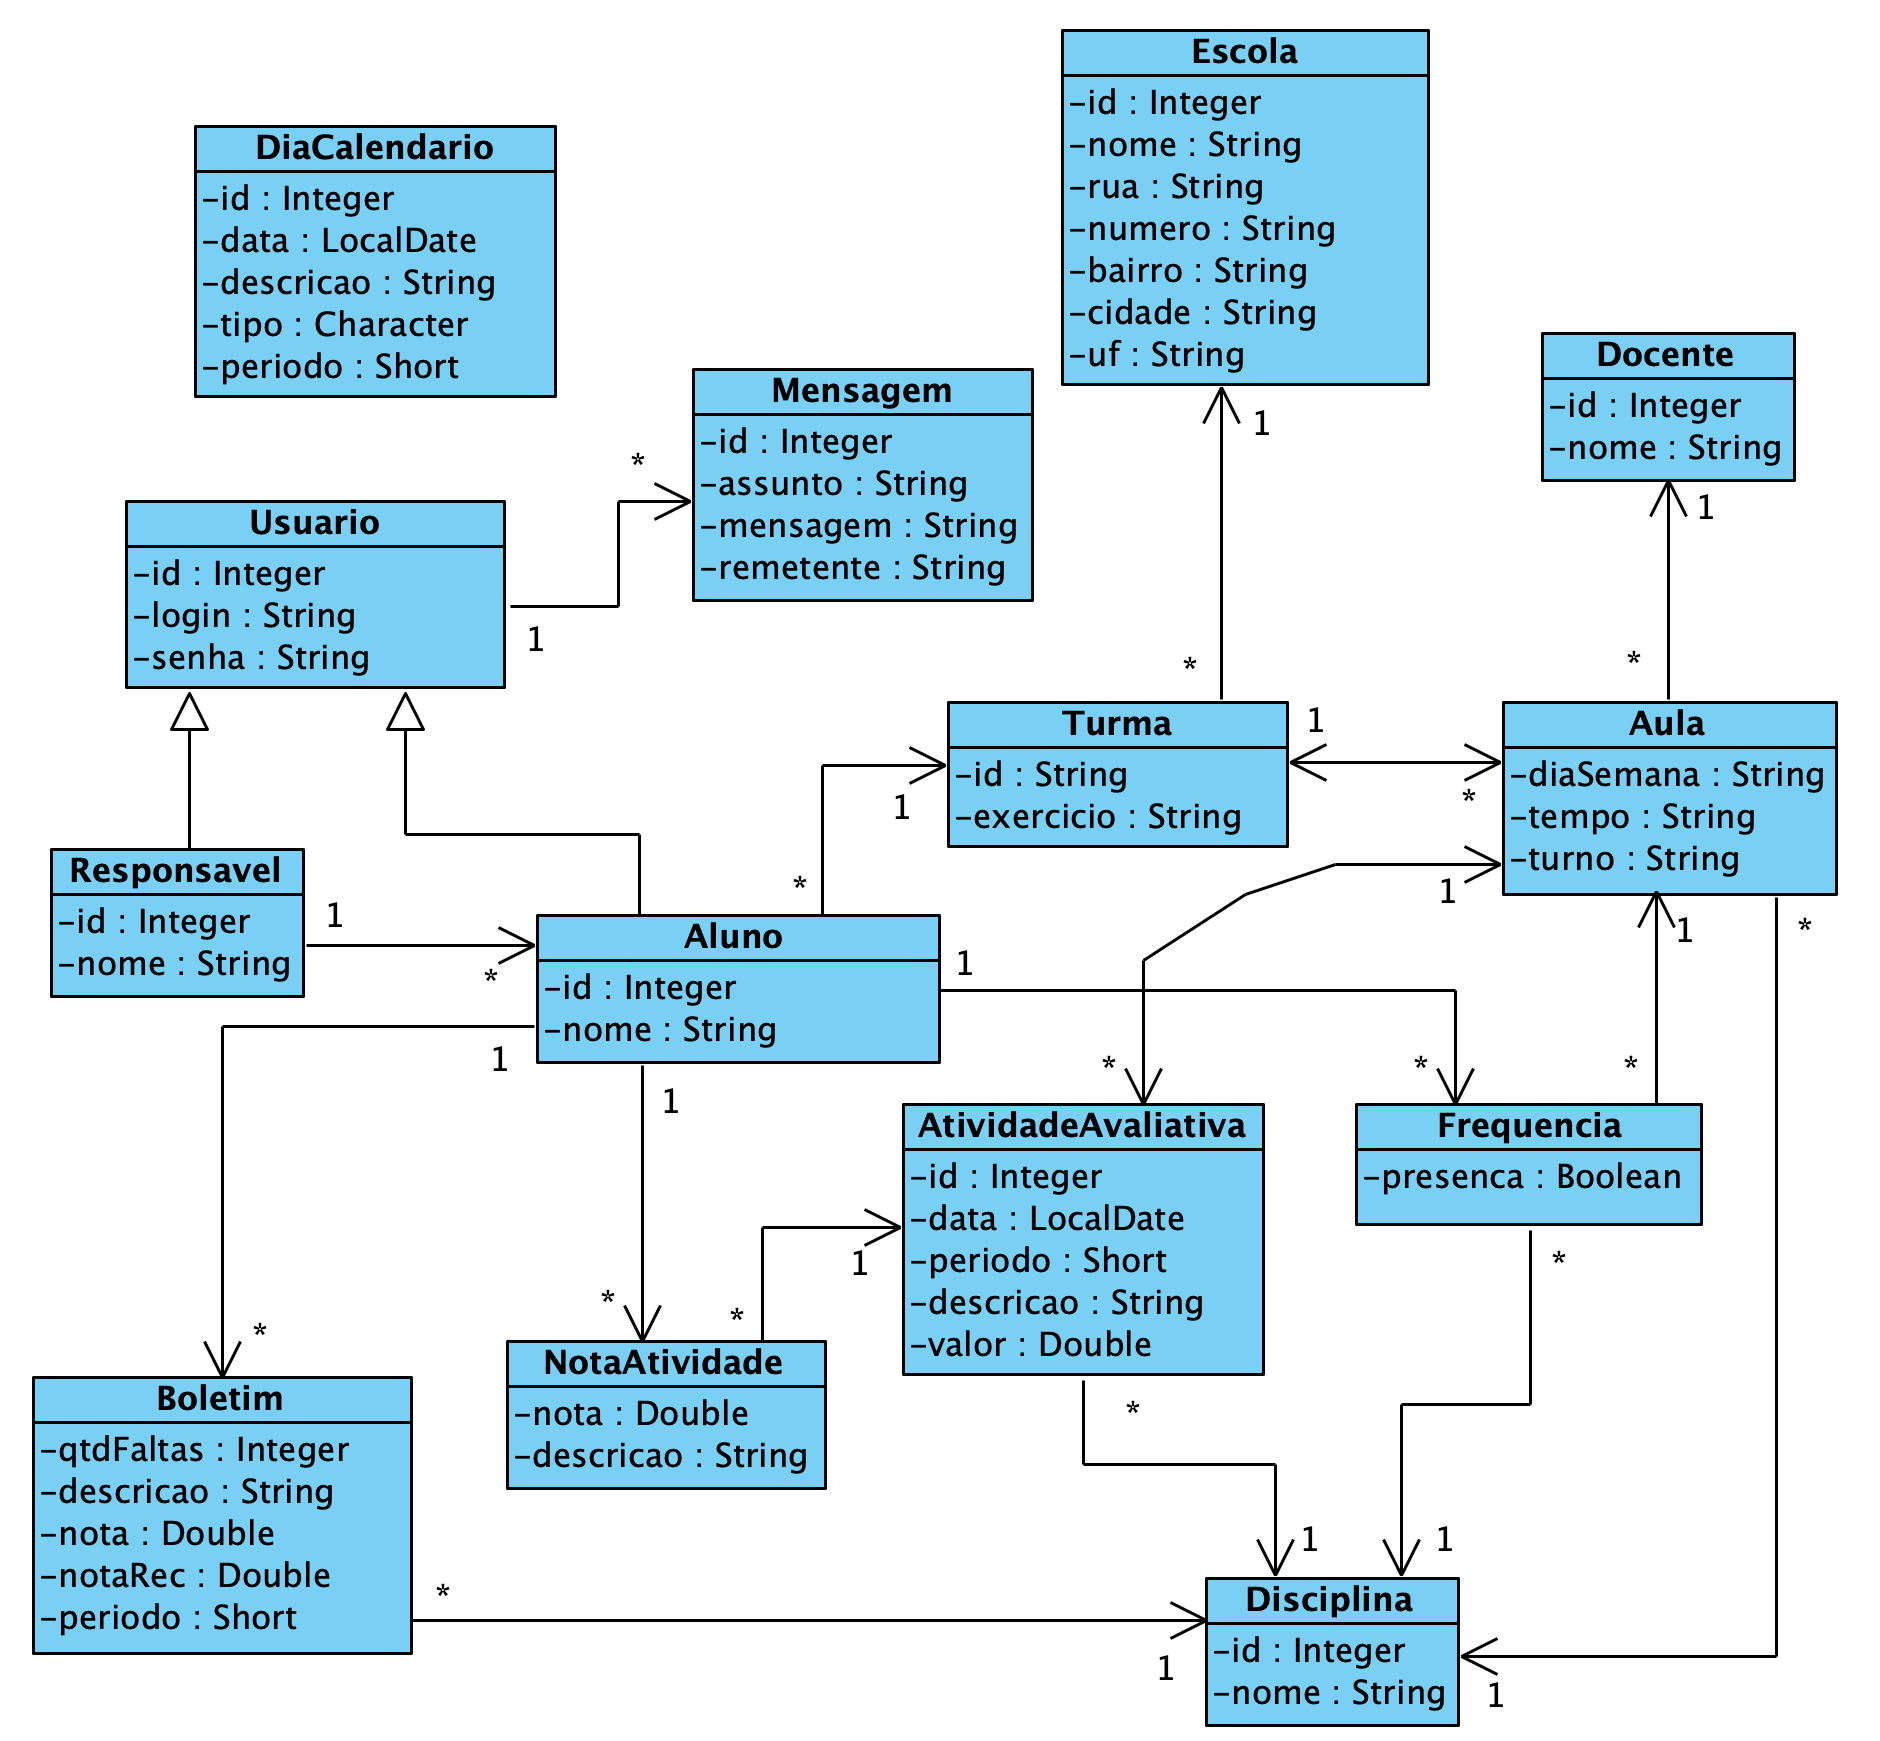
\includegraphics[width=16cm]{resources/classes_projeto.png} % leia abaixo
	\label{figura:diagrama_classe}
	\captionsetup{singlelinecheck = false, format= hang, justification=raggedright, labelsep=space, width=16cm}
	\caption*{\footnotesize Fonte: O Autor.}
\end{figure}

\subsection{Implementar}

\subsubsection{\textit{Web Service Restful}}

A implementação do \textit{web service} foi realizada utilizando a linguagem Java 1.8, e o \textit{framework Spring Boot} na versão 2.1.0. Foi utilizado o IDE \textit{Netbeans} 11.1 como ferramenta para codificação desta etapa. A organização do código da aplicação se dispõe em pacotes, tal como mostra a tabela \ref{tabela:webservice_package}.

\begin{table}[H]
    \small
	\centering
	\caption{Organização de pacotes do \textit{web service}.}
	\renewcommand{\arraystretch}{1.5}
	\begin{tabular}{>{\centering}m{1.5in} >{\centering\arraybackslash}m{2.0in}}
	    \hline
		\multicolumn{1}{c|}{\textbf{Pacote}} 
		& \multicolumn{1}{c}{\textbf{Descrição}}\\
		\hline
		model & Classes de modelo  \\
		service & Classes de serviço, para eventuais regras de negócio \\
		resource & Classes controladoras, que recebem e respondem chamadas ao \textit{web service} \\
		repository & Classes de acesso ao banco \\
		\hline
	\end{tabular}
	\label{tabela:webservice_package}
	\captionsetup{singlelinecheck = false, format= hang, justification=raggedright, labelsep=space, width=9.8cm}
	\caption*{\footnotesize Fonte: O Autor.}
\end{table}

A tabela \ref{tabela:webservice_servicos} apresenta o mapeamento de todos os serviços disponibilizados, especificando as URI de acesso, bem como seus respectivos métodos, tipos de retorno e descrições:

\begin{table}[H]
    \small
	\centering
	\caption{Mapeamento dos serviços do \textit{web service}.}
	\renewcommand{\arraystretch}{1.5}
	\begin{tabular}{>{\centering}m{1.8in} >{\centering}m{0.5in} >{\centering}m{1.35in} >{\centering\arraybackslash}m{1.95in}}
	    \hline
		\multicolumn{1}{c|}{\textbf{URI}} 
		& \multicolumn{1}{c|}{\textbf{Método}}
		& \multicolumn{1}{c|}{\textbf{Retorno}}
		& \multicolumn{1}{c}{\textbf{Descrição}}\\
		\hline
		/login & POST & - & Realiza login através das credenciais do usuário \\
		/aluno/alun/\{id\}/\{ano\} & GET & List<Aluno> & Busca um aluno por id e ano letivo \\
		/resp/\{id\}/\{ano\} & GET & List<Aluno> & Busca alunos por id do responsável e ano letivo \\
		/aluno/grade/\{id\} & GET & List<HorarioAula> & Busca aulas de uma grade horária por id do aluno \\
		/ativ/\{id\}/\{per\}/\{disc\} & GET & List<Atividade> & Busca atividades avaliativas por id do aluno, período e id da disciplina \\
		/ativ/\{id\}/\{per\} & GET & List<Disciplina> & Busca disciplinas de atividades avaliativas por id do aluno e período \\
		/aluno/boletim/\{id\}/\{per\} & GET & List<Boletim> & Busca boletins por id do aluno e período \\
		/freq/\{id\}/\{per\}/\{disc\}/total & GET & List<Frequencia> & Busca frequências por id do aluno, periodo e id da disciplina \\
		/freq/\{id\}/\{per\}/\{disc\}/total & GET & Integer & Busca total de frequências por id do aluno, periodo e id da disciplina \\
		/freq/\{id\}/\{per\} & GET & List<Disciplina> & Busca disciplinas de frequências por id do aluno e período \\
		/freq/\{id\}/\{per\}/total & GET & Integer & Busca total de faltas por id do aluno e período \\
		/cale/\{ano\} & GET & List<DiaCalendario> & Busca dias do calendário acadêmico por ano letivo \\
		/usuario/msg/\{id\} & GET & List<Mensagem> & Busca mensagens pelo id do usuário \\
		/resp/count & POST & - & Envia quantidade de cliques realizada pelo usuário com perfil de responsável \\
		\hline
	\end{tabular}
	\label{tabela:webservice_servicos}
	\captionsetup{singlelinecheck = false, format= hang, justification=raggedright, font=footnotesize, labelsep=space}
	\caption*{\footnotesize Fonte: O Autor.}
\end{table}

\subsubsection{Aplicativo Mobile}

O aplicativo \textit{mobile} foi implementado utilizando a linguagem \textit{Typescript}, através do \textit{framework} de desenvolvimento \textit{Ionic}, na versão 4. Foi utilizado o editor de texto \textit{Visual Studio Code} para a codificação desta etapa. A tabela \ref{tabela:app_organizacao} demonstra a organização básica dos principais diretórios do projeto, bem como suas respectivas descrições: 

\renewcommand{\arraystretch}{1.5}
\begin{table}[H]
    \small
	\centering
	\caption{Organização de Diretórios do Aplicativo \textit{Mobile}.}
	\label{tabela:app_organizacao}
	\begin{tabular}{c l}
	    \hline
		\multicolumn{1}{l|}{\textbf{Diretório}} & \multicolumn{1}{c}{\textbf{Descrição}}\\
		\hline
		models & Classes de mapeamento de dados retornados pela API  \\
		pages & Telas do aplicativo \\
		services & Classes de acesso ao \textit{web service} \\
		\hline
	\end{tabular}
	\captionsetup{singlelinecheck = false, format= hang, justification=raggedright, labelsep=space, width=11.9cm}
	\caption*{\footnotesize Fonte: O Autor.}
\end{table}
\renewcommand{\arraystretch}{1}

A seguir serão apresentadas as telas implementadas para as funcionalidades definidas no escopo do projeto:

\begin{itemize}
	\item Login (figura \ref{figura:login}): tela de \textit{login} do aplicativo;
	\item Menu Principal (figura \ref{figura:menu_principal}): contém opções de acesso para funcionalidades gerais do sistema e dados básicos do perfil do usuário logado;
	\item Listagem de alunos (figura \ref{figura:lista_alunos}): disponível apenas para usuários com perfil de responsável, esta funcionalidade lista todos os alunos vinculados ao perfil logado, permitindo o acesso aos dados de todos os alunos listados;
	\item Perfil do aluno (figura \ref{figura:perfil_aluno}): contém informações gerais sobre um aluno, bem como as opções de acesso aos dados acadêmicos do mesmo;
	\item Dias da grade horária (figura \ref{figura:grade_dias}): quando o usuário seleciona a função grade horária, a partir do perfil de um aluno (figura \ref{figura:perfil_aluno}), são listados todos os dias disponíveis em que há horários registrados com aulas para o aluno;
	\item Grade horária por dia (figura \ref{figura:grade}): ao selecionar um dia específico na tela representada pela figura \ref{figura:grade_dias}, são mostrados os horários registrados com aulas para o aluno por tempo, indicando a disciplina e o docente respectivos;
	\item Atividades avaliativas (figura \ref{figura:ativ_aval}): lista atividades avaliativas programadas por trimestre, bem como seus dados respectivos;
	\item Boletim Trimestral (figura \ref{figura:boletim}): exibe o boletim de um aluno dado um trimestre selecionado, com suas devidas disciplinas, notas e faltas;
	\item Listagem de frequências (figura \ref{figura:freq}): lista frequências do aluno por trimestre selecionado, indicando o conteúdo ministrado no dia e a quantidade de faltas;
	\item Calendário acadêmico (figura \ref{figura:calendario}): exibe todas as datas definidas para um ano letivo;
	\item Listagem de mensagens (figura \ref{figura:lista_mensagem}): lista mensagens enviadas para o usuário, mostrando se existe alguma mensagem ainda não lida;
	\item Mensagem visualizada (figura \ref{figura:mensagem}): mostra o conteúdo de uma mensagem, bem como o remetente e o assunto da mesma;
\end{itemize}

\begin{figure}[H]
    \begin{minipage}[b]{0.45\linewidth}
        \caption{Tela de Login.}
    	\centering % para centralizarmos a figura
    	\shadowbox{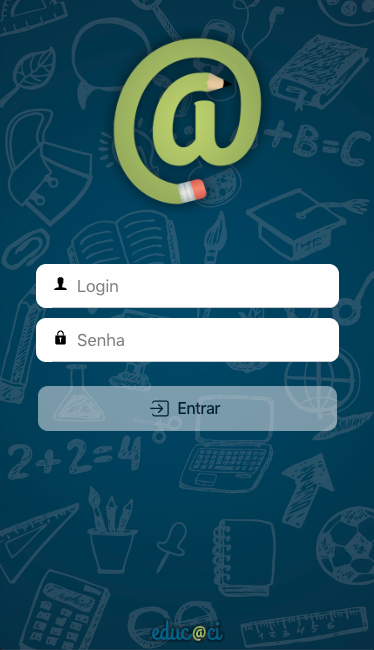
\includegraphics[width=5.7cm]{resources/prints_app/login.png}} % leia abaixo
    	\label{figura:login}
    	\captionsetup{singlelinecheck = false, format= hang, justification=raggedright, labelsep=space, width=6.2cm}
    	\caption*{\footnotesize Fonte: O Autor.}
    \end{minipage}
    \hspace{0.5cm}
    \begin{minipage}[b]{0.45\linewidth}
        \caption{Menu principal.}
    	\centering % para centralizarmos a figura
    	\shadowbox{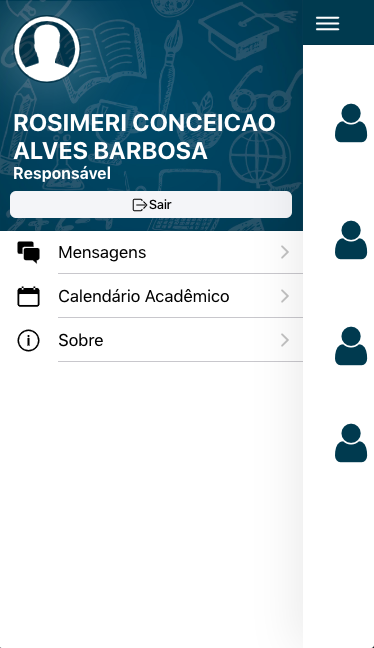
\includegraphics[width=5.7cm]{resources/prints_app/menu_principal.png}} % leia abaixo
    	\label{figura:menu_principal}
    	\captionsetup{singlelinecheck = false, format= hang, justification=raggedright, labelsep=space, width=6.2cm}
    	\caption*{\footnotesize Fonte: O Autor.}
    \end{minipage}
\end{figure}

\begin{figure}[H]
    \begin{minipage}[b]{0.45\linewidth}
        \caption{Listagem de alunos.}
    	\centering % para centralizarmos a figura
    	\shadowbox{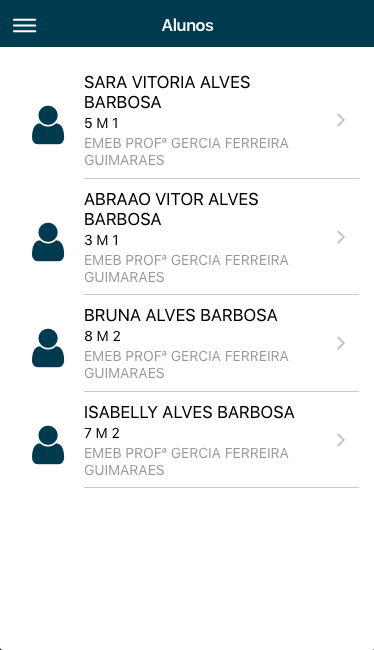
\includegraphics[width=5.7cm]{resources/prints_app/listagem_alunos.png}} % leia abaixo
    	\label{figura:lista_alunos}
    	\captionsetup{singlelinecheck = false, format= hang, justification=raggedright, labelsep=space, width=6.2cm}
    	\caption*{\footnotesize Fonte: O Autor.}
    \end{minipage}
    \hspace{0.5cm}
    \begin{minipage}[b]{0.45\linewidth}
        \caption{Perfil do aluno.}
    	\centering % para centralizarmos a figura
    	\shadowbox{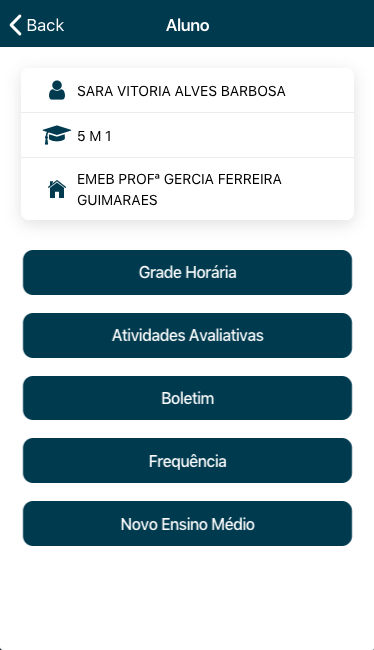
\includegraphics[width=5.7cm]{resources/prints_app/perfil_aluno.png}} % leia abaixo
    	\label{figura:perfil_aluno}
    	\captionsetup{singlelinecheck = false, format= hang, justification=raggedright, labelsep=space, width=6.2cm}
    	\caption*{\footnotesize Fonte: O Autor.}
    \end{minipage}
\end{figure}

\begin{figure}[H]
    \begin{minipage}[b]{0.45\linewidth}
        \caption{Dias da grade horária.}
    	\centering % para centralizarmos a figura
    	\shadowbox{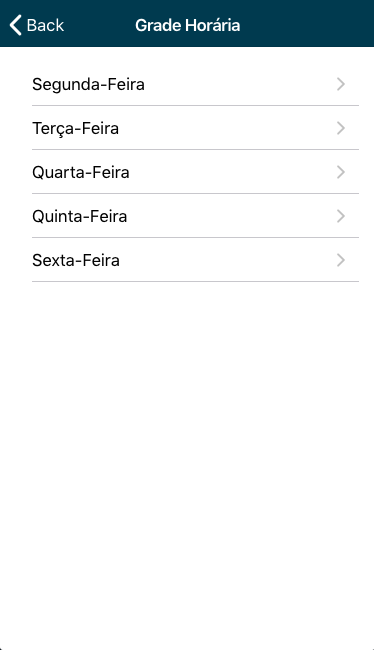
\includegraphics[width=5.7cm]{resources/prints_app/grade_horaria1.png}} % leia abaixo
    	\label{figura:grade_dias}
    	\captionsetup{singlelinecheck = false, format= hang, justification=raggedright, labelsep=space, width=6.2cm}
    	\caption*{\footnotesize Fonte: O Autor.}
    \end{minipage}
    \hspace{0.5cm}
    \begin{minipage}[b]{0.45\linewidth}
        \caption{Grade horária por dia.}
    	\centering % para centralizarmos a figura
    	\shadowbox{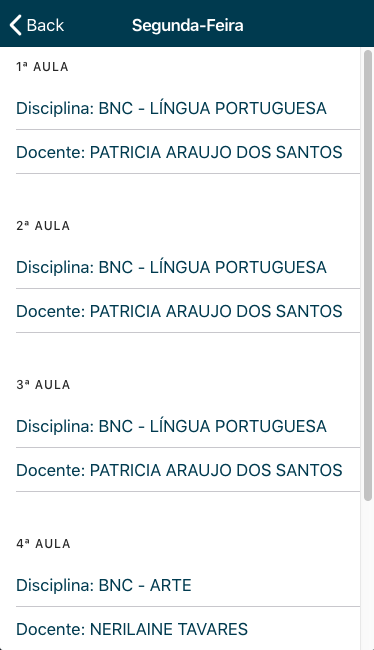
\includegraphics[width=5.7cm]{resources/prints_app/grade_horaria2.png}} % leia abaixo
    	\label{figura:grade}
    	\captionsetup{singlelinecheck = false, format= hang, justification=raggedright, labelsep=space, width=6.2cm}
    	\caption*{\footnotesize Fonte: O Autor.}
    \end{minipage}
\end{figure}

\begin{figure}[H]
    \begin{minipage}[b]{0.45\linewidth}
        \caption{Atividades avaliativas.}
    	\centering % para centralizarmos a figura
    	\shadowbox{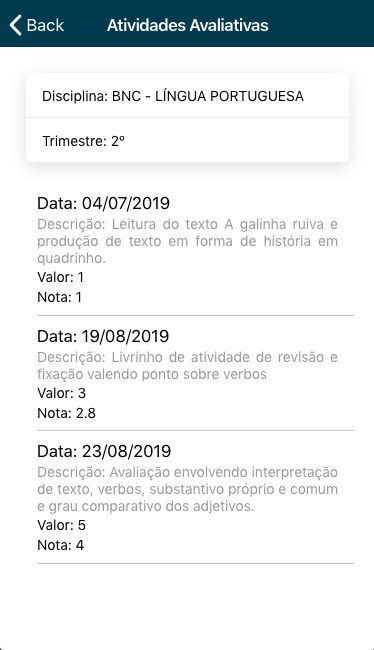
\includegraphics[width=5.7cm]{resources/prints_app/atividades_avaliativas.png}} % leia abaixo
    	\label{figura:ativ_aval}
    	\captionsetup{singlelinecheck = false, format= hang, justification=raggedright, labelsep=space, width=6.2cm}
    	\caption*{\footnotesize Fonte: O Autor.}
    \end{minipage}
    \hspace{0.5cm}
    \begin{minipage}[b]{0.45\linewidth}
        \caption{Boletim trimestral.}
    	\centering % para centralizarmos a figura
    	\shadowbox{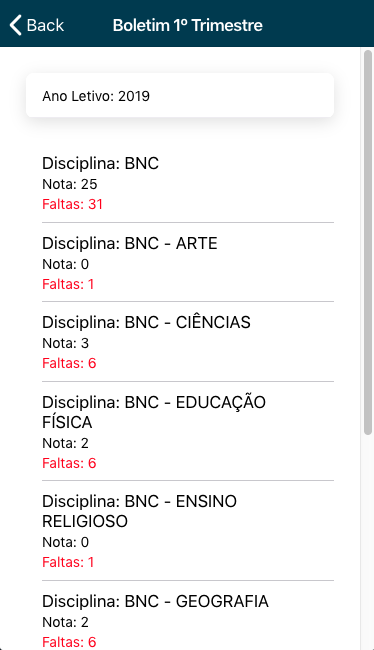
\includegraphics[width=5.7cm]{resources/prints_app/boletim.png}} % leia abaixo
    	\label{figura:boletim}
    	\captionsetup{singlelinecheck = false, format= hang, justification=raggedright, labelsep=space, width=6.2cm}
    	\caption*{\footnotesize Fonte: O Autor.}
    \end{minipage}
\end{figure}

\begin{figure}[H]
    \begin{minipage}[b]{0.45\linewidth}
        \caption{Listagem de frequências.}
    	\centering % para centralizarmos a figura
    	\shadowbox{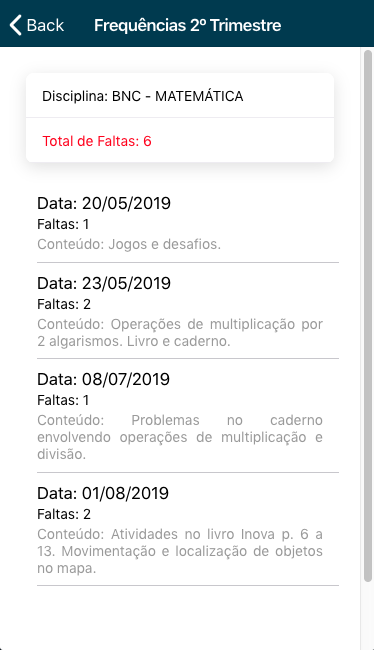
\includegraphics[width=5.7cm]{resources/prints_app/frequencias.png}} % leia abaixo
    	\label{figura:freq}
    	\captionsetup{singlelinecheck = false, format= hang, justification=raggedright, labelsep=space, width=6.2cm}
    	\caption*{\footnotesize Fonte: O Autor.}
    \end{minipage}
    \hspace{0.5cm}
    \begin{minipage}[b]{0.45\linewidth}
        \caption{Calendário acadêmico.}
    	\centering % para centralizarmos a figura
    	\shadowbox{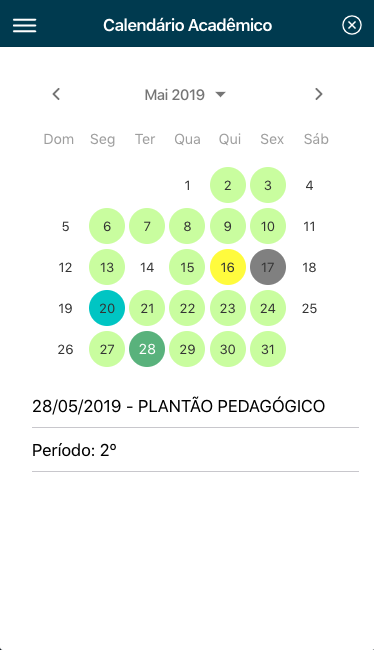
\includegraphics[width=5.7cm]{resources/prints_app/calendario_academico.png}} % leia abaixo
    	\label{figura:calendario}
    	\captionsetup{singlelinecheck = false, format= hang, justification=raggedright, labelsep=space, width=6.2cm}
    	\caption*{\footnotesize Fonte: O Autor.}
    \end{minipage}
\end{figure}

\begin{figure}[H]
    \begin{minipage}[b]{0.45\linewidth}
        \caption{Listagem de mensagens.}
    	\centering % para centralizarmos a figura
    	\shadowbox{
\includegraphics[width=5.7cm]{resources/prints_app/lista_mensagens.png}} % leia abaixo
    	\label{figura:lista_mensagem}
    	\captionsetup{singlelinecheck = false, format= hang, justification=raggedright, labelsep=space, width=6.2cm}
    	\caption*{\footnotesize Fonte: O Autor.}
    \end{minipage}
    \hspace{0.5cm}
    \begin{minipage}[b]{0.45\linewidth}
        \caption{Mensagem visualizada.}
    	\centering % para centralizarmos a figura
    	\shadowbox{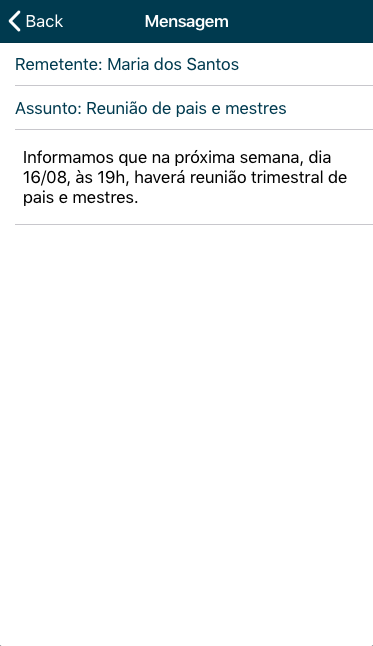
\includegraphics[width=5.7cm]{resources/prints_app/mensagem.png}} % leia abaixo
    	\label{figura:mensagem}
    	\captionsetup{singlelinecheck = false, format= hang, justification=raggedright, labelsep=space, width=6.2cm}
    	\caption*{\footnotesize Fonte: O Autor.}
    \end{minipage}
\end{figure}

\subsection{Testar}

Foram realizados testes de validação \cite{pressman2016engenharia} no aplicativo pela empresa parceira e por escolas piloto do município definidas pela mesma. Neste processo foram testadas todas as funcionalidades do aplicativo em busca de inconsistências. Ao encontrar uma eventual inconsistência, a empresa realizava a comunicação através de mensagens de e-mail, sendo realizadas as devidas correções logo após. Durante este período, a empresa parceira proporcionou um ambiente para testes através de uma base de dados de teste idêntica a base de produção utilizada pelo software de gestão educacional do município.

\subsection{Implantar}

A implantação do \textit{web service} foi realizada na infraestrutura da empresa parceira, utilizando o servidor \textit{Payara Web Server} na versão 1.192. A publicação do aplicativo foi realizada através da conta da empresa parceira na loja de aplicativos da plataforma \textit{Android}. A publicação para a plataforma \textit{IOS} já se encontra em processo de andamento.

\section{Módulo de classificação baseado em Redes Neurais}

A Implementação do módulo baseado em redes neurais foi implementada utilizando a biblioteca \textit{Weka}, na versão 3.8.3. Para tal, foram executados os seguintes passos no processo de construção:

\subsection{Selecionar variáveis para o treinamento da rede}

Nesta etapa foi realizada, sob auxílio de um pedagogo, dentre um conjunto de quarenta variáveis disponíveis na base de dados cedida, a seleção de dezenove variáveis para a realização do treinamento da rede. Durante o processo, foram realizadas 2 reuniões com o pedagogo. As variáveis selecionadas estão dispostas a seguir, conforme mostra tabela \ref{tabela:variaveis}. 

\begin{table}[H]
    \small
	\centering
	\caption{Variáveis utilizadas no treinamento da rede.}
	\renewcommand{\arraystretch}{1.5}
	\begin{tabular}{>{\centering}m{1.8in} >{\centering\arraybackslash}m{4.2in}}
	    \hline
		\multicolumn{1}{c|}{\textbf{Variável}} 
		& \multicolumn{1}{c}{\textbf{Descrição}}\\
		\hline
		grau\textunderscore pai & Grau de escolaridade do pai \\
		grau\textunderscore mae & Grau de escolaridade da mãe \\
		duracao\textunderscore gestacao & Duração da gestação do aluno \\
		autismo & Indica se o aluno é portador de autismo \\
		superdotacao & Indica se o aluno possui superdotação \\
		bolsa\textunderscore familia & Indica se o aluno é participante programa Bolsa Família \\
		escola & Indica a escola onde o aluno estuda \\
		escola\textunderscore internet & Indica se a escola possui internet \\
		escola\textunderscore integral & Indica se a escola possui turno integral \\
		pai\textunderscore vivo & Indica se o pai é vivo \\
		mae\textunderscore viva & Indica se a mão é viva \\
		sexo & Indica o sexo do aluno \\
		percentual\textunderscore frequência & Indica o percentual de frequência do aluno considerando toda a sua vida acadêmica como estudante na rede de ensino \\
		media\textunderscore português & média das notas do aluno na disciplina de português (considerando todos os anos registrados) \\
		media\textunderscore matematica & média das notas do aluno na disciplina de matemática (considerando todos os anos registrados) \\
		media\textunderscore historia & média das notas do aluno na disciplina de história (considerando todos os anos registrados) \\
		media\textunderscore geografia & média das notas do aluno na disciplina de geografia (considerando todos os anos registrados) \\
		media\textunderscore ciências & média das notas do aluno na disciplina de ciências (considerando todos os anos registrados) \\
		cliques\textunderscore responsavel & quantidade de cliques ou interações realizadas pelo responsável do aluno junto ao aplicativo \\
		\hline
	\end{tabular}
	\label{tabela:variaveis}
	\captionsetup{singlelinecheck = false, format= hang, justification=raggedright, font=footnotesize, labelsep=space}
	\caption*{\footnotesize Fonte: O Autor.}
\end{table}

\subsection{Preparar o arquivo de treinamento}

Nesta etapa foi produzido um arquivo utilizado pelo \textit{Weka} com extensão ARFF, contendo as variáveis de treinamento selecionadas na etapa anterior, as classes para classificação, e dados de cem alunos já classificados. Tais dados são utilizados como exemplo de treinamento para a rede, que utiliza aprendizagem supervisionada. Devido ao fato do novo ensino médio ainda não ter sido implantado, os exemplos de alunos classificados inseridos no arquivo de treinamento foram simulados, porém atendendo aos requisitos das variáveis selecionadas na etapa anterior.

\subsection{Realizar o treinamento da rede}

O processo de treinamento da rede foi realizado utilizando a ferramenta \textit{Weka Explorer}, que realiza a leitura do arquivo de treinamento, exibindo as informações do mesmo de forma gráfica. Como algoritmo de treinamento foi utilizado o \textit{Multilayer Perceptron}. No decorrer do treinamento foram utilizadas várias configurações objetivando aumentar a taxa de acerto de classificação da rede. A tabela \ref{tabela:configuracoes} demonstra algumas configurações utilizadas no processo de treinamento da rede.

\begin{table}[H]
    \small
	\centering
	\caption{Configurações prévias de treinamento utilizadas.}
	\renewcommand{\arraystretch}{1.8}
	\begin{tabular}{>{\centering}m{1.2in} >{\centering}m{1.5in} >{\centering}m{1.2in} >{\centering}m{1.2in} >{\centering\arraybackslash}m{1.2in}}
	    \hline
		\multicolumn{1}{c|}{\textbf{\parbox{1.1in}{\centering Nº de camadas ocultas\footnotemark[1]}}}
		& \multicolumn{1}{c|}{\textbf{\parbox{1.5in}{\centering Nº de neurônios por camada oculta\footnotemark[1]}}}
		& \multicolumn{1}{c|}{\textbf{\parbox{1.05in}{\centering Taxa de aprendizagem\footnotemark[2]}}}
		& \multicolumn{1}{c|}{\textbf{\parbox{0.7in}{\centering Tempo de treino\footnotemark[3]}}}
		& \multicolumn{1}{c}{\textbf{\parbox{1.1in}{\centering Taxa de acerto obtida (\%)}}}\\
	    \hline
	\end{tabular}
	\renewcommand{\arraystretch}{1.5}
	\begin{tabular}{>{\centering}m{1.1in} >{\centering}m{1.5in} >{\centering}m{1.05in} >{\centering}m{0.7in} >{\centering\arraybackslash}m{1.1in}}
	    1 & 24 & 0.3 & 500 & 94 \\
	    1 & 20 & 0.6 & 500 & 92 \\
	    1 & 12 & 0.3 & 500 & 94 \\
	    1 & 12 & 0.3 & 180 & 94 \\
	    2 & 4, 23 & 0.3 & 500 & 93 \\
	    2 & 12, 20 & 0.3 & 500 & 91 \\
	    2 & 12, 20 & 0.6 & 500 & 89 \\
	    2 & 12, 20 & 0.3 & 300 & 91 \\
	    3 & 12, 20, 30 & 0.3 & 500 & 86 \\
	    3 & 12, 20, 30 & 0.6 & 300 & 91 \\
	    3 & 12, 20, 30 & 0.3 & 800 & 87 \\
	    3 & 12, 20, 30 & 0.6 & 800 & 89 \\
		\hline
	\end{tabular}
	\label{tabela:configuracoes}
	\captionsetup{singlelinecheck = false, format= hang, justification=raggedright, labelsep=space, width=6.3in}
	\caption*{\footnotesize Fonte: O Autor.}
\end{table}

\footnotetext[1]{As camadas ocultas são as camadas dispostas entre a camada de entrada e a camada de saída da rede \cite{hagan1996neural}.} 
\footnotetext[2]{Regula a quantidade de atualizações nos pesos das variáveis \cite{morariu2018weka}.} 
\footnotetext[3]{Representa uma quantidade de iterações executadas, indicando quando o processo de treino deve parar de ser executado \cite{morariu2018weka}.}

Foram testadas configurações com uma, duas e três camadas escondidas, buscando obter melhores resultados. A configuração final utilizada foi a que atingiu a maior taxa de acerto com os menores valores de configuração, sendo eles: uma camada oculta com 12 neurônios; taxa de aprendizagem de 0.3; e tempo de treino 180, chegando a uma taxa de acerto de classificação obtida de 94\%. As figuras \ref{figura:resultado} e \ref{figura:rede} demonstram, respectivamente, o resultado do treinamento realizado e a disposição gráfica da configuração final da rede.

% \begin{figure}[H]
% 	\caption{Configuração final do treinamento.}
% 	\centering % para centralizarmos a figura
% 	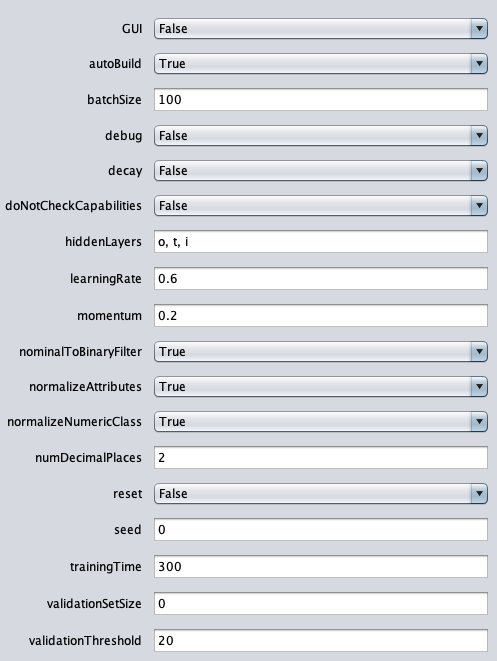
\includegraphics[width=11cm]{resources/treinamento_weka.png} % leia abaixo
% 	\label{figura:treinamento}
% 	\captionsetup{singlelinecheck = false, format= hang, justification=raggedright, labelsep=space, width=11cm}
% 	\caption*{\footnotesize Fonte: O Autor.}
% \end{figure}

\begin{figure}[H]
	\caption{Resultado do treinamento.}
	\centering % para centralizarmos a figura
	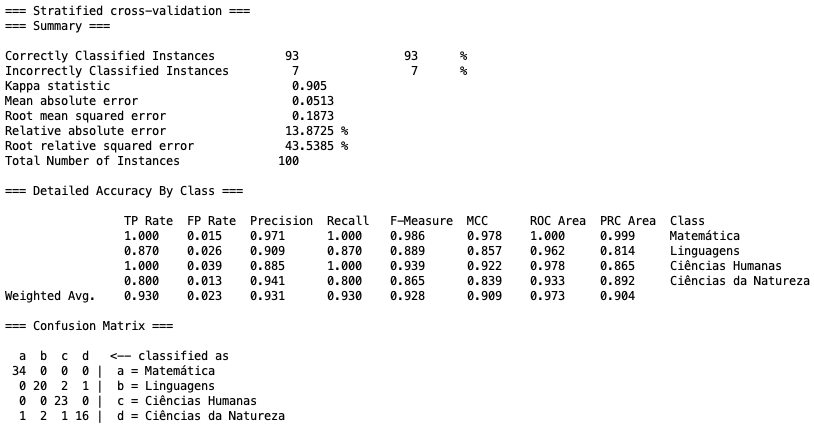
\includegraphics[width=16cm]{resources/resultado_treinamento.png} % leia abaixo
	\label{figura:resultado}
	\captionsetup{singlelinecheck = false, format= hang, justification=raggedright, labelsep=space, width=16cm}
	\caption*{\footnotesize Fonte: O Autor.}
\end{figure}

\begin{figure}[H]
	\caption{Disposição da rede em camadas.}
	\centering % para centralizarmos a figura
	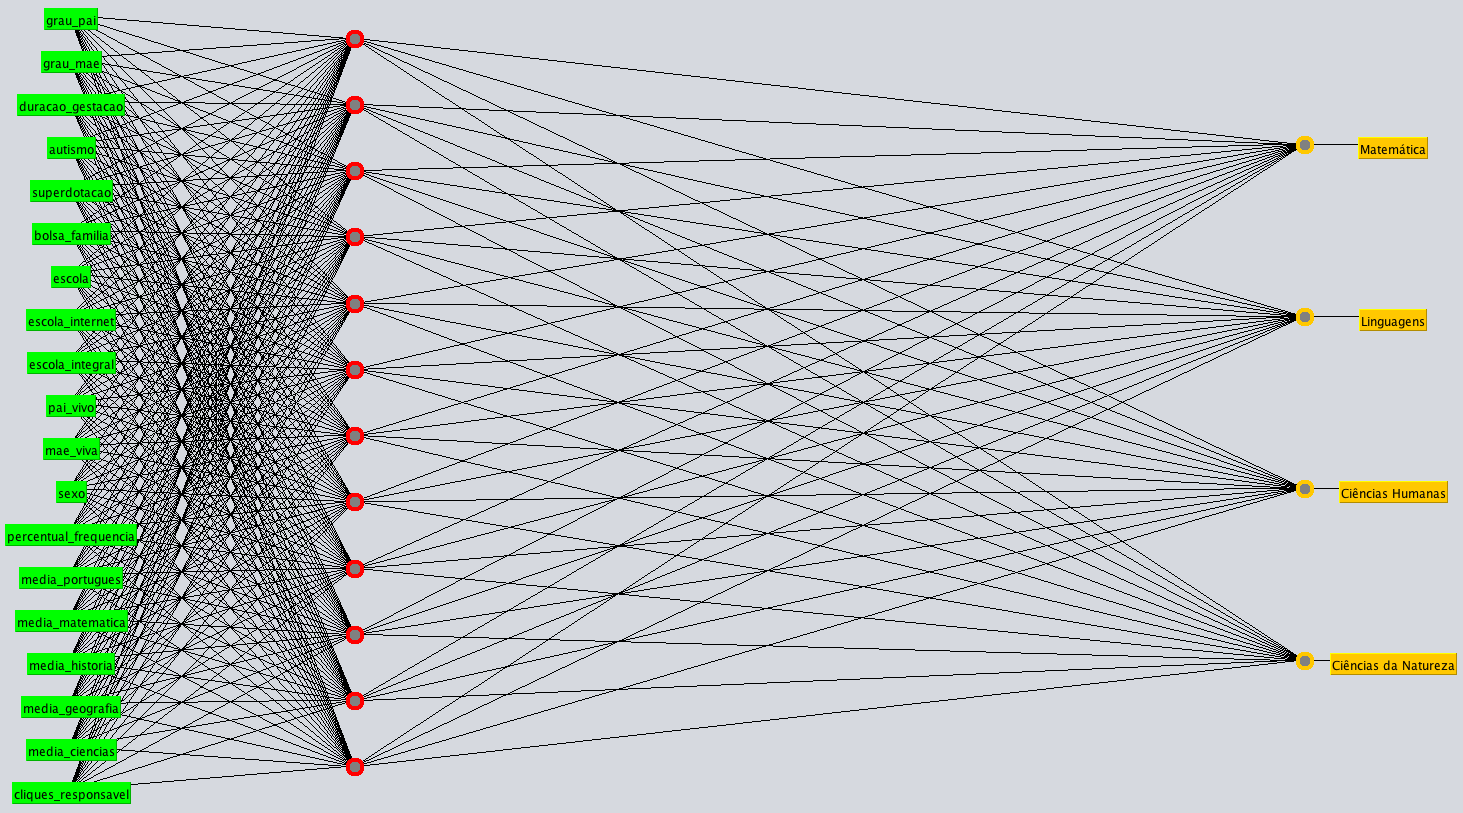
\includegraphics[width=16cm]{resources/rede.png} % leia abaixo
	\label{figura:rede}
	\captionsetup{singlelinecheck = false, format= hang, justification=raggedright, labelsep=space, width=16cm}
	\caption*{\footnotesize Fonte: O Autor.}
\end{figure}

\subsection{Integrar o módulo junto ao web service e ao aplicativo}

Nesta fase foi realizada a integração da rede treinada com o \textit{web service}, através da incorporação ao projeto do \textit{Weka} como biblioteca, do arquivo de treinamento, e das configurações de treinamento. O mapeamento do serviço responsável por esta funcionalidade é representado pela tabela \ref{tabela:webservice_treinamento}. O resultado gerado pelo serviço fornece uma distribuição de porcentagem entre as áreas de conhecimento, sendo utilizada pelo aplicativo na geração de um gráfico indicativo, que apresenta uma porcentagem para cada área de conhecimento do novo ensino médio, tal como mostra a figura \ref{figura:distribuicao}.

\begin{table}[H]
    \small
	\centering
	\caption{Mapeamento do serviço de classificação.}
	\renewcommand{\arraystretch}{1.5}
	\begin{tabular}{>{\centering}m{1.3in} >{\centering}m{0.5in} >{\centering}m{0.6in} >{\centering\arraybackslash}m{3.2in}}
	    \hline
		\multicolumn{1}{c|}{\textbf{URI}} 
		& \multicolumn{1}{c|}{\textbf{Método}}
		& \multicolumn{1}{c|}{\textbf{Retorno}}
		& \multicolumn{1}{c}{\textbf{Descrição}}\\
		\hline
		/aluno/classify/\{id\} & GET & double[] & Retorna uma distribuição de porcentagem entre as áreas de conhecimento do novo ensino médio dado como parâmetro o id de um aluno \\
		\hline
	\end{tabular}
	\label{tabela:webservice_treinamento}
	\captionsetup{singlelinecheck = false, format= hang, justification=raggedright, font=footnotesize, labelsep=space}
	\caption*{\footnotesize Fonte: O Autor.}
\end{table}

\begin{figure}[H]
    \caption{Distribuição de porcentagens por áreas de conhecimento do novo ensino médio.}
	\centering % para centralizarmos a figura
	\shadowbox{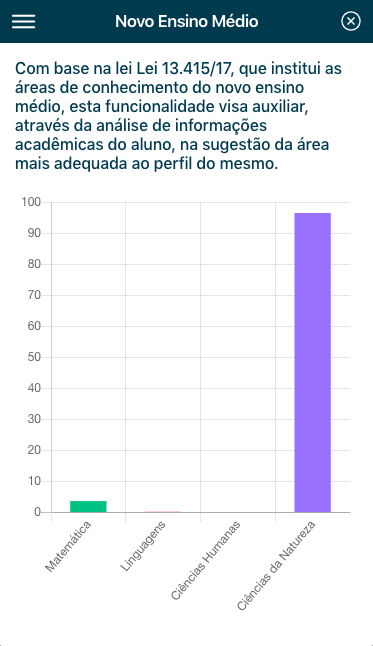
\includegraphics[width=6cm]{resources/prints_app/classificacao.png}} % leia abaixo
	\label{figura:distribuicao}
	\captionsetup{singlelinecheck = false, format= hang, justification=raggedright, labelsep=space, width=6.5cm}
	\caption*{\footnotesize Fonte: O Autor.}
\end{figure}

\section{Avaliação do Software}

Foi realizado avaliação do \textit{software} construído através de pesquisa realizada com 37 alunos do ensino médio integrado do Ifes Campus Cachoeiro de Itapemirim. Para tal, foi utilizado um formulário baseado na metodologia definida por \citeonline{reeves1993user}, que avalia aspectos de interface gráfica do \textit{software} produzido. A figura \ref{figura:avaliacao} demonstra os resultados da pesquisa:

\begin{figure}[H]
	\caption{Avaliação do aplicativo por alunos do ensino médio do IFES Campus Cachoeiro.}
	\centering % para centralizarmos a figura
	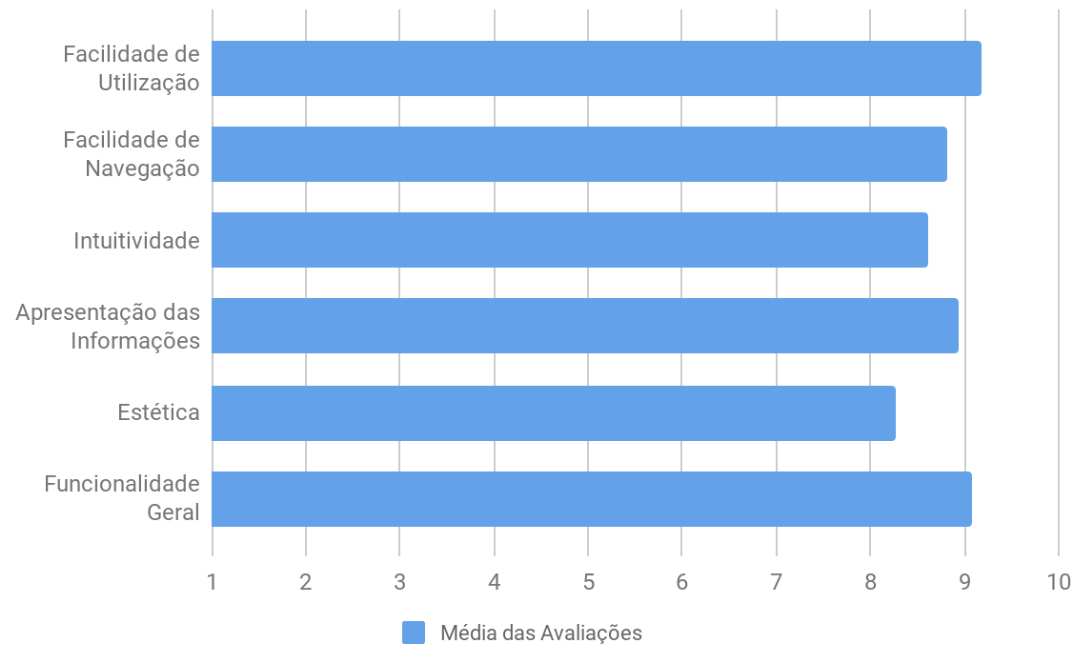
\includegraphics[width=15cm]{resources/pesquisa_avaliacao.png} % leia abaixo
	\label{figura:avaliacao}
	\captionsetup{singlelinecheck = false, format= hang, justification=raggedright, labelsep=space, width=15cm}
	\caption*{\footnotesize Fonte: O Autor.}
\end{figure}

Foi realizado também a validação do aplicativo através de apresentações em três oportunidades: na empresa parceira, com a presença dos responsáveis da empresa; na secretaria de educação do município em questão, com a presença dos gestores das escolas piloto; e por apresentação realizada em uma das escolas piloto.